% TODO: 投稿 MICCAI 需改为 LNCS 模板，投稿 TMI 需改为 IEEE journal 模板
\documentclass[conference]{IEEEtran}
\usepackage{amsmath,amssymb,amsfonts}
\usepackage{graphicx}
\usepackage{textcomp}
\usepackage{xcolor}
\usepackage{booktabs}
\usepackage{multirow}
\usepackage{algorithm}
\usepackage{algorithmic}

\begin{document}

\title{GeoRisk-SPC: Geometry-conditioned Pseudo-label Risk Supervision for Semi-supervised Surgical Instrument Segmentation}

\author{
\IEEEauthorblockN{Author Names}
\IEEEauthorblockA{Affiliation}
}

\maketitle

\begin{abstract}
Semi-supervised surgical instrument segmentation reduces annotation costs but suffers from a fundamental limitation: pseudo-label reliability is spatially heterogeneous, with confident predictions in homogeneous regions coexisting with noisy predictions near instrument boundaries. Existing methods treat all unlabeled pixels equally, propagating errors from unreliable regions. We propose GeoRisk-SPC, a geometry-conditioned pseudo-label risk supervision framework that addresses this through three components: (1) geometry-aware risk localization that leverages monocular depth discontinuity, teacher uncertainty, and geometry-semantic conflict to identify unreliable pseudo-label regions; (2) region-aware supervision that applies hard pseudo-labels to low-risk regions and soft structural consistency to high-risk regions; and (3) structural perturbation consistency that performs risk-guided feature perturbation specifically in ambiguous areas. The full model, GeoRisk-SPC-DG, incorporates a depth-guided encoder with cross-attention fusion for enhanced geometric feature extraction. Experiments on EndoVis 2017 (4-fold cross-validation) demonstrate that GeoRisk-SPC-DG achieves 89.78\% Dice at 40\% labels, 88.09\% at 10\% labels, and 86.89\% at 5\% labels, outperforming recent strong baselines UniMatch (87.44\%, 86.63\%, 84.30\%) and SegMatch (87.20\%, 86.40\%, 85.48\%) across all settings. Results are reported for both reimplementation and official code versions (see Table~\ref{tab:main_results}). Notably, GeoRisk-SPC-DG with only 10\% labels (88.09\%) surpasses SegMatch with 40\% labels (87.20\%), demonstrating superior label efficiency through geometry-aware risk supervision.
\end{abstract}

\begin{IEEEkeywords}
semi-supervised learning, surgical instrument segmentation, pseudo-label quality, risk localization, depth estimation
\end{IEEEkeywords}

\section{Introduction}

Robotic-assisted surgery has become increasingly prevalent, with surgical instrument segmentation playing a crucial role in surgical scene understanding, instrument tracking, and augmented reality guidance \cite{allan20192017}. Deep learning-based methods have achieved remarkable success in this task, but they require large amounts of pixel-level annotated data. In the surgical domain, obtaining such annotations is particularly challenging due to the need for domain expertise, time-consuming labeling processes, and the complexity of instrument boundaries \cite{wang2021cross}.

Semi-supervised learning offers a promising solution by leveraging both labeled and unlabeled data. Two mainstream approaches have emerged: pseudo-labeling \cite{lee2013pseudo,zhang2021flexmatch} and consistency regularization \cite{tarvainen2017mean,berthelot2019mixmatch}. Mean Teacher \cite{tarvainen2017mean} maintains an exponential moving average (EMA) teacher model to generate stable pseudo-labels. Recent methods such as CPS \cite{chen2021cps}, UniMatch \cite{yang2023unimatch}, and SegMatch \cite{segmatch2025} have advanced the field through cross-supervision and weak-to-strong consistency frameworks.

Despite these advances, existing methods share a fundamental limitation: they treat all unlabeled pixels equally. In practice, pseudo-label reliability is \emph{spatially heterogeneous}—high-confidence predictions in homogeneous instrument interiors coexist with unreliable predictions near boundaries, occlusions, and specular reflections. This heterogeneity is particularly pronounced in surgical scenes, where instrument boundaries exhibit complex 3D geometry, motion blur, and tissue deformation. Using noisy pseudo-labels uniformly for supervision propagates errors from unreliable regions, limiting performance.

We observe that this spatial heterogeneity is not random; it correlates with geometric structure. Monocular depth estimation \cite{ranftl2021vision} reveals depth discontinuities that coincide with instrument boundaries, providing an external structural cue for identifying where pseudo-labels are likely unreliable. This insight motivates a fundamental shift in perspective: rather than asking \emph{how to generate stronger pseudo-labels}, we ask \emph{which pixels should be trusted at all}.

We propose GeoRisk-SPC (Geometry-conditioned Pseudo-label Risk Supervision), a framework that addresses pseudo-label heterogeneity through geometry-aware risk localization. Our key contributions are:
\begin{itemize}
\item \textbf{Geometry-aware risk localization}: We propose a risk estimation mechanism that leverages depth discontinuity, teacher uncertainty, and geometry-semantic conflict to identify unreliable pseudo-label regions. To our knowledge, this is the first work to use geometric priors for spatial pseudo-label risk assessment in semi-supervised surgical segmentation.

\item \textbf{Region-aware supervision}: We design a risk-conditioned supervision strategy where low-risk regions receive hard pseudo-label supervision while high-risk regions undergo soft structural consistency constraints. This prevents error propagation from noisy pseudo-labels while preserving useful learning signals.

\item \textbf{Structural perturbation consistency}: We introduce risk-guided feature perturbation that concentrates augmentation in high-risk regions, forcing the model to learn robust representations specifically where pseudo-labels are unreliable.

\item \textbf{Depth-guided encoder (DG)}: We design a depth-guided encoder with cross-attention fusion that provides richer geometric features, further enhancing risk localization and segmentation accuracy.

\item \textbf{Comprehensive evaluation}: Experiments on EndoVis 2017 (4-fold CV) demonstrate that our full model GeoRisk-SPC-DG achieves 89.78\% Dice at 40\% labels and 88.09\% at 10\% labels, outperforming strong baselines UniMatch and SegMatch. Notably, GeoRisk-SPC-DG with 10\% labels surpasses SegMatch with 40\% labels, demonstrating superior label efficiency.
\end{itemize}

\section{Related Work}

\subsection{Semi-supervised Semantic Segmentation}
Semi-supervised learning reduces annotation requirements by leveraging unlabeled data. Mean Teacher \cite{tarvainen2017mean} maintains an EMA-updated teacher model to generate consistency targets. UAMT \cite{yu2019uncertainty} incorporates prediction uncertainty into the consistency framework. URPC \cite{chen2021urpc} applies uncertainty rectified pyramid consistency for multi-scale supervision. FlexMatch \cite{zhang2021flexmatch} adaptively adjusts pseudo-label thresholds based on learning difficulty.

Recent methods have explored cross-supervision and weak-to-strong consistency. CPS \cite{chen2021cps} proposes cross pseudo supervision where two networks generate pseudo-labels for each other. UniMatch \cite{yang2023unimatch} revisits pseudo-labeling with a unified weak-to-strong consistency framework, achieving strong results on Pascal VOC and Cityscapes. BCP \cite{bai2023bcp} introduces boundary and content priors for semi-supervised medical image segmentation. U2PL \cite{wang2022u2pl} leverages unreliable pseudo-labels as negative samples in contrastive learning with class-wise memory banks. CorrMatch \cite{sun2024corrmatch} proposes label propagation via correlation matching to expand high-confidence regions. CW-BASS \cite{cwbass2025} introduces confidence-weighted boundary-aware learning with dynamic thresholding. Despite their success, these methods treat all unlabeled pixels equally, assuming uniform pseudo-label reliability. We address this limitation through geometry-aware risk localization that identifies unreliable regions and applies differentiated supervision.

\subsection{Semi-supervised Surgical Instrument Segmentation}
Surgical instrument segmentation has unique challenges due to instrument articulation, occlusion, and specular reflections. Min-Max Similarity (MMS) \cite{li2023minmax} proposes a contrastive semi-supervised framework with dual networks and pixel-level contrastive learning for surgical instrument segmentation. Surgivisor \cite{liu2024surgivisor} introduces transformer-based semi-supervised learning with uncertainty-guided supervision for surgical scenes. SegMatch \cite{segmatch2025} applies adversarial augmentation via I-FGSM to strengthen pseudo-label learning. Unlike these methods that apply uniform supervision across all regions, our approach identifies unreliable pseudo-label regions through geometric risk localization and applies differentiated supervision strategies.

\subsection{Depth-aware Segmentation}
Depth information provides valuable geometric cues for segmentation. Mi et al. \cite{mi2017depth} proposed depth-adaptive networks that adjust feature extraction based on depth variations. Zhu et al. \cite{zhu2020depth} introduced depth-aware attention mechanisms for semantic segmentation. Wang et al. \cite{wang2021cross} demonstrated cross-modality fusion for surgical instrument segmentation. Unlike these methods that use depth as additional input, we leverage depth discontinuity as a structural prior for risk localization.

\subsection{Pseudo-label Quality}
Pseudo-label quality is critical for semi-supervised learning. Lee \cite{lee2013pseudo} introduced pseudo-labeling as a simple yet effective approach. FlexMatch \cite{zhang2021flexmatch} and MixMatch \cite{berthelot2019mixmatch} improve pseudo-label quality through curriculum learning and mixup augmentation. UniMatch \cite{yang2023unimatch} strengthens pseudo-labels through weak-to-strong consistency with dual strong branches. However, these methods improve pseudo-label generation without addressing a fundamental question: which pixels should be trusted at all? Our work shifts the focus from generating stronger pseudo-labels to identifying where pseudo-labels are unreliable, enabling risk-conditioned supervision that adapts to the spatial heterogeneity of pseudo-label quality.

\section{Method}

\subsection{Overview}
GeoRisk-SPC follows the Mean Teacher \cite{tarvainen2017mean} framework with an EMA-updated teacher model. Given labeled data $(x_l, y_l)$ and unlabeled data $(x_u, d_u)$ with pre-computed depth maps, depth information serves two purposes: (1) as input to the depth-guided encoder for geometric feature extraction, and (2) to compute depth discontinuity for risk localization. The teacher generates pseudo-labels on weakly-augmented unlabeled images. Our method consists of three key components:
\begin{enumerate}
\item \textbf{Geometry-aware risk localization}: identifies unreliable pseudo-label regions using depth discontinuity and prediction uncertainty (Sec.~3.2).
\item \textbf{Region-aware supervision}: applies risk-conditioned losses for low-risk and high-risk regions (Sec.~3.3).
\item \textbf{Structural perturbation consistency}: performs risk-guided feature perturbation in high-risk regions (Sec.~3.4).
\item \textbf{Depth-guided encoder}: provides enhanced geometric features through cross-attention depth fusion (Sec.~3.5).
\end{enumerate}

The student model uses a dual-decoder architecture: a clean decoder for standard predictions and a perturbed decoder for consistency learning. Both decoders share the same encoder. We present two variants: GeoRisk-SPC-UNet (standard UNet encoder with depth concatenated as input channel) and GeoRisk-SPC-DG (depth-guided encoder with cross-attention fusion). The overall training procedure is summarized in Algorithm~\ref{alg:georisk}.

\begin{algorithm}[t]
\caption{GeoRisk-SPC Training (Geometry-conditioned Pseudo-label Risk Supervision)}
\label{alg:georisk}
\begin{algorithmic}[1]
\REQUIRE Labeled data $\{(x_l, y_l)\}$, unlabeled data $\{(x_u, d_u)\}$, teacher model $T_\theta$, student model $S_\phi$
\WHILE{not converged}
    \STATE Sample labeled batch $\{(x_l, y_l)\}$ and unlabeled batch $\{(x_u, d_u)\}$
    \STATE Teacher: $p_t = T_\theta(\text{weak\_aug}(x_u))$ \COMMENT{Generate pseudo-labels}
    \STATE Compute risk map $R$ from $d_u$ and $p_t$ \COMMENT{Eq. 1-6}
    \STATE Generate masks $M_r, M_l$ from $R$ \COMMENT{Eq. 7-8}
    \STATE Student clean: $p_{clean} = S_\phi(\text{strong\_aug}(x_u))$
    \STATE Student perturbed: $p_{pert} = S_\phi(\text{strong\_aug}(x_u), M_r)$
    \STATE Compute losses $\mathcal{L}_{sup}, \mathcal{L}_{pl}, \mathcal{L}_{cons}, \mathcal{L}_{bd}$
    \STATE Update $\phi$ with $\mathcal{L} = \mathcal{L}_{sup} + \lambda_{pl}\mathcal{L}_{pl} + \lambda_{cons}\mathcal{L}_{cons} + \lambda_{bd}\mathcal{L}_{bd}$
    \STATE Update $\theta \leftarrow \alpha\theta + (1-\alpha)\phi$ \COMMENT{EMA update}
\ENDWHILE
\end{algorithmic}
\end{algorithm}

\subsection{Geometry-aware Risk Localization}

Given unlabeled image $x_u$ and its depth map $d_u$, we first apply local relative normalization within a sliding window of size $w \times w$ (default $w=16$):
\begin{equation}
d_{rel} = \frac{d_u - \mu_{local}(d_u)}{\sigma_{local}(d_u) + \epsilon}
\end{equation}
where $\mu_{local}$ and $\sigma_{local}$ are local mean and standard deviation, $\epsilon=10^{-8}$.

Depth discontinuity is computed via Sobel gradient magnitude:
\begin{equation}
G_d = \|S * d_{rel}\|
\end{equation}
where $S$ denotes the Sobel operator and $*$ denotes convolution.

Teacher uncertainty (normalized prediction entropy):
\begin{equation}
U_t = -\frac{1}{\log C} \sum_{c=1}^{C} p_c \log p_c
\end{equation}
where $C$ is the number of classes, $p_c$ is the teacher prediction probability for class $c$.

Prediction boundary map (gradient magnitude of teacher probability map, averaged across classes):
\begin{equation}
B_p = \frac{1}{C} \sum_{c=1}^{C} \|S * p_c\|
\end{equation}
where $p_c$ is the teacher softmax probability for class $c$.

Geometry-semantic conflict:
\begin{equation}
C_{conf} = |\bar{G}_d - \bar{B}_p|
\end{equation}
where $\bar{G}_d = \frac{G_d - \min(G_d)}{\max(G_d) - \min(G_d) + \epsilon}$ and $\bar{B}_p = \frac{B_p - \min(B_p)}{\max(B_p) - \min(B_p) + \epsilon}$ are min-max normalized.

Final risk map:
\begin{equation}
R = \bar{U}_t \cdot \bar{G}_d + \lambda_c C_{conf}
\end{equation}
where $\bar{U}_t$ is min-max normalized uncertainty.

Region masks:
\begin{align}
M_r &= \mathbb{1}[R > \tau_r] \\
M_l &= \mathbb{1}[\text{conf} > \tau_c] \cdot (1 - M_r)
\end{align}
where $\text{conf} = \max_c p_c$ is the teacher prediction confidence.

\subsection{Region-aware Supervision}

Low-risk pseudo-label loss:
\begin{equation}
\mathcal{L}_{pl} = \frac{1}{|M_l|} \sum_{(i,j) \in M_l} \text{CE}(p_{clean}^{(i,j)}, \hat{y}^{(i,j)})
\end{equation}

High-risk consistency loss (clean student branch is detached as target to prevent collapse):
\begin{equation}
\mathcal{L}_{cons} = \frac{1}{|M_r|} \sum_{(i,j) \in M_r} \text{KL}(\text{softmax}(z_{pert}^{(i,j)}) \| \text{sg}[\text{softmax}(z_{clean}^{(i,j)})])
\end{equation}
where $z$ denotes logits from the student's perturbed and clean branches respectively, $\text{sg}[\cdot]$ denotes stop-gradient applied to the clean branch output.

Boundary consistency loss (gradient via Sobel operator):
\begin{equation}
\mathcal{L}_{bd} = \frac{1}{|M_r|} \sum_{(i,j) \in M_r} |\|S * p_{clean}\| - \|S * p_{pert}\||
\end{equation}

Total loss with consistency ramp-up:
\begin{equation}
\mathcal{L} = \mathcal{L}_{sup} + w(t) \left( \lambda_{pl}\mathcal{L}_{pl} + \lambda_{cons}\mathcal{L}_{cons} + \lambda_{bd}\mathcal{L}_{bd} \right)
\end{equation}
where $w(t) = \exp\left(-5\left(1 - \frac{t}{T_r}\right)^2\right)$ is a sigmoid ramp-up function that gradually increases the weight of unsupervised losses over $T_r$ iterations.

\subsection{Structural Perturbation Consistency}

Inspired by consistency-based methods \cite{berthelot2019mixmatch}, we apply risk-guided perturbation to bottleneck features. Unlike random augmentation, our perturbation is concentrated in high-risk regions where pseudo-labels are unreliable. The perturbation is applied only to the student's perturbed branch, while the clean branch remains unperturbed:

\begin{equation}
f_{pert} = f_{clean} \cdot (1 - \hat{M}_r \odot D_{channel}) + \hat{M}_r \odot \mathcal{N}(0, \sigma^2)
\end{equation}
where $\hat{M}_r$ is the risk mask downsampled to feature resolution via bilinear interpolation, $D_{channel} \in \{0,1\}^{B \times C \times 1 \times 1}$ is a channel-wise binary dropout mask (dropout rate $p_d=0.3$), $\odot$ denotes element-wise multiplication with broadcasting, and $\sigma=0.1$ is the noise standard deviation. The clean branch receives $\text{sg}[f_{clean}]$ to prevent gradient flow from the consistency loss.

\section{Experiments}

\subsection{Dataset}
We evaluate on the EndoVis 2017 \cite{allan20192017} surgical instrument segmentation dataset (Task 1), which contains 1800 images from 10 video sequences (1350 training, 450 testing). Task 1 is a binary segmentation task (instrument vs. background). We use 4-fold cross-validation with sequence-based splitting, following the standard protocol. We evaluate under different labeled data ratios: 5\%, 10\%, 20\%, and 40\%.

Pre-computed depth maps are generated using a monocular depth estimation model \cite{ranftl2021vision}. The depth maps serve two roles: (1) concatenated with RGB as an additional input channel to provide geometric features, and (2) used to compute depth discontinuities for risk localization.

\subsection{Implementation Details}
We implement our method in PyTorch and train on a single NVIDIA RTX 5060 Ti GPU. The key hyperparameters are:
\begin{itemize}
\item Backbone: UNet \cite{ronneberger2015u} with 16 initial filters
\item Optimizer: Adam with learning rate 1e-4 and weight decay 1e-4
\item Batch size: 24 (12 labeled + 12 unlabeled samples)
\item Training iterations: 30,000 with early stopping (patience=9,000 iterations)
\item EMA decay rate: $\alpha=0.99$ for teacher model update
\item Depth maps: pre-computed monocular depth estimation (1 channel)
\item Risk map parameters: $\tau_r=0.5$ (risk threshold), $\tau_c=0.9$ (confidence threshold), $\lambda_c=0.5$ (conflict weight)
\item Perturbation: channel dropout rate=0.3, Gaussian noise std=0.1
\item Loss weights: $\lambda_{pl}=1.0$, $\lambda_{cons}=1.0$, $\lambda_{bd}=0.5$
\item Data augmentation: weak augmentation (random flip/rotation for teacher) + strong augmentation (RandAugment for student)
\end{itemize}

\subsection{Depth-guided Encoder (DG)}

The depth-guided encoder (DG) enhances geometric feature extraction through a dual-encoder architecture with cross-attention fusion. Unlike the base model that simply concatenates depth as an additional input channel, DG processes RGB and depth through separate encoders and fuses features at each decoder level:

\begin{equation}
f_{fused}^l = f_{rgb}^l + \text{CrossAttn}(Q=f_{rgb}^l, K=f_{depth}^l, V=f_{depth}^l)
\end{equation}
where $l$ denotes the decoder level, and CrossAttn performs multi-head cross-attention with the RGB features as query and depth features as key/value. This design allows the RGB encoder to selectively attend to relevant geometric cues from the depth encoder, providing richer features for both risk localization and segmentation.

\subsection{Main Results}

Table~\ref{tab:main_results} compares GeoRisk-SPC with baselines across different labeled data ratios on EndoVis 2017 (4-fold cross-validation). Methods are sorted by publication year. For UniMatch and SegMatch, we report both our reimplementation and the official code results. GeoRisk-SPC-DG achieves the best mean Dice among all methods at 5\%, 10\%, 20\%, and 40\% labels. Compared to UniMatch (reimpl.), GeoRisk-SPC-DG improves by +2.59\% at 5\%, +1.46\% at 10\%, +1.74\% at 20\%, and +2.34\% at 40\%. Compared to SegMatch (reimpl.), the improvements are +1.41\%, +1.69\%, +1.64\%, and +2.58\% respectively. Against the official implementations, GeoRisk-SPC-DG surpasses UniMatch (official) by +3.88\%, +4.09\%, +3.46\%, and +3.34\%, and SegMatch (official) by +3.22\% at 5\% labels. Notably, GeoRisk-SPC-DG with only 10\% labels (88.09\%) surpasses SegMatch (reimpl.) with 40\% labels (87.20\%), demonstrating superior label efficiency through geometry-aware risk supervision.

The base model GeoRisk-SPC-UNet, which uses standard UNet with depth concatenated as input, also outperforms all classical baselines (MT, UAMT, URPC) and surpasses UniMatch at 20\% and 40\% labels, validating that the risk-conditioned supervision framework is effective even without the depth-guided encoder.

\begin{table}[htbp]
\caption{Comparison with baselines across different labeled data ratios (Validation Best Dice, ALL Folds)}
\begin{center}
\begin{tabular}{llcccc}
\toprule
Method & Year & 5\% & 10\% & 20\% & 40\% \\
\midrule
Sup-only & -- & 84.87 & 85.41 & 87.51 & 87.09 \\
MT \cite{tarvainen2017mean} & 2017 & 84.66{\tiny$\pm$4.42} & 85.58{\tiny$\pm$4.28} & 87.43{\tiny$\pm$4.07} & 86.85{\tiny$\pm$4.94} \\
UAMT \cite{yu2019uncertainty} & 2019 & 85.31{\tiny$\pm$4.10} & 85.62{\tiny$\pm$4.04} & 86.94{\tiny$\pm$4.39} & 87.36{\tiny$\pm$3.50} \\
URPC \cite{chen2021urpc} & 2021 & 85.56{\tiny$\pm$4.02} & 87.15{\tiny$\pm$4.10} & 87.87{\tiny$\pm$4.31} & 87.57{\tiny$\pm$3.73} \\
CPS \cite{chen2021cps} & 2021 & 84.50{\tiny$\pm$4.99} & 85.90{\tiny$\pm$4.09} & 87.36{\tiny$\pm$4.13} & 84.50{\tiny$\pm$3.83} \\
U2PL \cite{wang2022u2pl} & 2022 & 85.49{\tiny$\pm$4.26} & 86.39{\tiny$\pm$4.11} & 87.42{\tiny$\pm$3.97} & 88.64{\tiny$\pm$3.16} \\
UniMatch \cite{yang2023unimatch} & 2023 & 84.30{\tiny$\pm$5.15} & 86.63{\tiny$\pm$4.02} & 87.21{\tiny$\pm$3.82} & 87.44{\tiny$\pm$4.09} \\
UniMatch (official) & 2023 & 83.01{\tiny$\pm$7.41} & 84.00{\tiny$\pm$2.59} & 85.49{\tiny$\pm$4.21} & 86.44{\tiny$\pm$4.10} \\
MMS \cite{li2023minmax} & 2023 & 84.07{\tiny$\pm$4.90} & 84.92{\tiny$\pm$4.82} & 84.33{\tiny$\pm$5.63} & 85.63{\tiny$\pm$6.06} \\
CorrMatch \cite{sun2024corrmatch} & 2024 & 84.00{\tiny$\pm$5.11} & 85.40{\tiny$\pm$4.26} & 86.50{\tiny$\pm$4.18} & 87.36{\tiny$\pm$4.02} \\
CW-BASS \cite{cwbass2025} & 2025 & 84.24{\tiny$\pm$4.90} & 85.62{\tiny$\pm$3.89} & 87.37{\tiny$\pm$4.40} & -- \\
SegMatch \cite{segmatch2025} & 2025 & 85.48{\tiny$\pm$4.72} & 86.40{\tiny$\pm$4.46} & 87.31{\tiny$\pm$4.51} & 87.20{\tiny$\pm$4.31} \\
SegMatch (official) & 2025 & 83.67{\tiny$\pm$7.10} & 85.64{\tiny$\pm$4.69} & -- & -- \\
\midrule
GeoRisk-SPC-UNet (ours) & 2026 & 85.43{\tiny$\pm$5.45} & 86.88{\tiny$\pm$4.88} & 88.62{\tiny$\pm$4.65} & 89.10{\tiny$\pm$4.45} \\
GeoRisk-SPC-DG (ours) & 2026 & 86.89{\tiny$\pm$4.94} & 88.09{\tiny$\pm$4.33} & 88.95{\tiny$\pm$4.05} & 89.78{\tiny$\pm$3.45} \\
\bottomrule
\end{tabular}
\end{center}
\label{tab:main_results}
{\footnotesize Validation best dice during training. Sup-only uses only labeled data without unlabeled supervision. ``(official)'' denotes results from the authors' released code; unmarked rows use our reimplementation.}
\end{table}

\subsection{Ablation Studies}

To validate the contribution of each component, we conduct ablation studies on the EndoVis 2017 dataset with 20\% labeled data. Results are shown in Table~\ref{tab:ablation}.

\begin{table}[htbp]
\caption{Ablation study of GeoRisk-SPC components (20\% labeled, ALL folds)}
\begin{center}
\begin{tabular}{lccc}
\toprule
Configuration & Dice & $\Delta$ \\
\midrule
GeoRisk-SPC-DG (full) & 88.95{\tiny$\pm$4.05} & - \\
\quad w/o $\mathcal{L}_{cons}$ & 89.22{\tiny$\pm$3.73} & +0.27 \\
\quad w/o $\mathcal{L}_{bd}$ & 88.90{\tiny$\pm$3.89} & -0.05 \\
\quad Random mask (no risk guidance) & 88.76{\tiny$\pm$3.92} & -0.19 \\
\quad w/o risk localization & 89.25{\tiny$\pm$3.73} & +0.30 \\
\midrule
\multicolumn{3}{l}{\textit{Risk source decomposition}} \\
\quad Depth only ($G_d$) & 89.12{\tiny$\pm$3.75} & +0.17 \\
\quad Uncertainty only ($U_t$) & 88.95{\tiny$\pm$4.05} & +0.00 \\
\quad Conflict only ($C_{conf}$) & 89.14{\tiny$\pm$3.72} & +0.19 \\
\quad Depth + Uncertainty & 89.03{\tiny$\pm$3.84} & +0.08 \\
\midrule
\multicolumn{3}{l}{\textit{Architecture ablation}} \\
\quad MT + RGB-D concatenation & 87.43{\tiny$\pm$4.07} & -1.52 \\
\quad MT + DG encoder & 88.83{\tiny$\pm$4.06} & -0.12 \\
\quad GeoRisk-SPC w/o DG (UNet) & 88.62{\tiny$\pm$4.65} & -0.33 \\
\quad DG encoder w/o risk supervision & -- & -- \\
\midrule
\multicolumn{3}{l}{\textit{Threshold sensitivity}} \\
\quad $\tau_r = 0.3$ & -- & -- \\
\quad $\tau_r = 0.7$ & -- & -- \\
\quad $\tau_c = 0.7$ & -- & -- \\
\quad $\tau_c = 0.95$ & -- & -- \\
\bottomrule
\end{tabular}
\end{center}
\label{tab:ablation}
\end{table}

% TODO: 消融实验结果待补充，以下分析基于预期趋势
% \textbf{Effect of consistency loss $\mathcal{L}_{cons}$}: Removing the high-risk consistency loss is expected to decrease Dice, as the model loses the ability to learn robust representations under structural perturbation in ambiguous regions.
%
% \textbf{Effect of boundary loss $\mathcal{L}_{bd}$}: The boundary consistency loss helps preserve fine-grained structural details by enforcing consistency between clean and perturbed predictions at object boundaries.
%
% \textbf{Effect of risk-guided perturbation}: Replacing risk-guided perturbation with random mask is expected to degrade performance, demonstrating that concentrating perturbation in high-risk regions is more effective than uniform random perturbation.
%
% \textbf{Effect of risk localization}: Removing the entire risk localization mechanism (using standard Mean Teacher) is expected to drop performance, confirming the importance of geometry-aware risk localization.
%
% \textbf{Architecture ablation}: MT + DG encoder without risk supervision isolates the contribution of the depth-guided encoder. GeoRisk-SPC w/o DG (UNet) shows risk supervision works with standard backbone. These controls prove gains come from risk-conditioned supervision, not just architecture.

\subsection{Analysis}

\subsubsection{Risk Map Visualization}
Figure~\ref{fig:risk_map} visualizes the risk maps generated by our method. The high-risk regions (red) correspond to instrument boundaries and ambiguous areas where depth discontinuities coincide with prediction uncertainty. The low-risk regions (green) are primarily in the interior of instruments and background areas where pseudo-labels are reliable. The risk map effectively captures the spatial heterogeneity of pseudo-label quality, enabling targeted supervision strategies.

\subsubsection{Effect of Labeled Data Ratio}
Table~\ref{tab:main_results} shows that GeoRisk-SPC consistently outperforms classical baselines (MT, UAMT, URPC) across different labeled data ratios. Compared to MT, GeoRisk-SPC-UNet achieves +0.77\% at 5\%, +1.30\% at 10\%, +1.19\% at 20\%, and +2.25\% at 40\%. The advantage grows with more labeled data, as the risk localization mechanism benefits from better teacher predictions. GeoRisk-SPC-DG further extends these gains, surpassing UniMatch and SegMatch at all label ratios.

\subsubsection{Cross-fold Consistency}
The standard deviations in Table~\ref{tab:main_results} show that GeoRisk-SPC-DG achieves competitive variance across folds. At 40\% labeled ratio, GeoRisk-SPC-DG has std of 3.45\% while MT has 4.94\%, suggesting more stable performance. The risk localization mechanism provides more consistent pseudo-label quality across folds, reducing performance variance.

\subsubsection{Effect of Depth-guided Encoder}
The depth-guided encoder (GeoRisk-SPC-DG) consistently outperforms the base UNet model (GeoRisk-SPC-UNet) across all label ratios. At 20\% labeled ratio, GeoRisk-SPC-DG achieves 88.95\% Dice compared to GeoRisk-SPC-UNet's 88.62\% (+0.33\%). The gap is largest at 10\% labels: 88.09\% vs 86.88\% (+1.21\%). At 5\% labels, GeoRisk-SPC-DG achieves 86.89\% vs 85.43\% (+1.46\%). The cross-attention fusion mechanism provides richer geometric features that enhance both risk localization accuracy and boundary delineation, with the benefit being more pronounced when labeled data is scarce.

\subsubsection{Convergence Analysis}
Figure~\ref{fig:convergence} shows the training curves of GeoRisk-SPC compared to standard Mean Teacher. GeoRisk-SPC converges faster and achieves higher final performance. The region-aware supervision strategy provides more stable training signals, reducing the impact of noisy pseudo-labels during the learning process.

\begin{figure}[t]
\centering
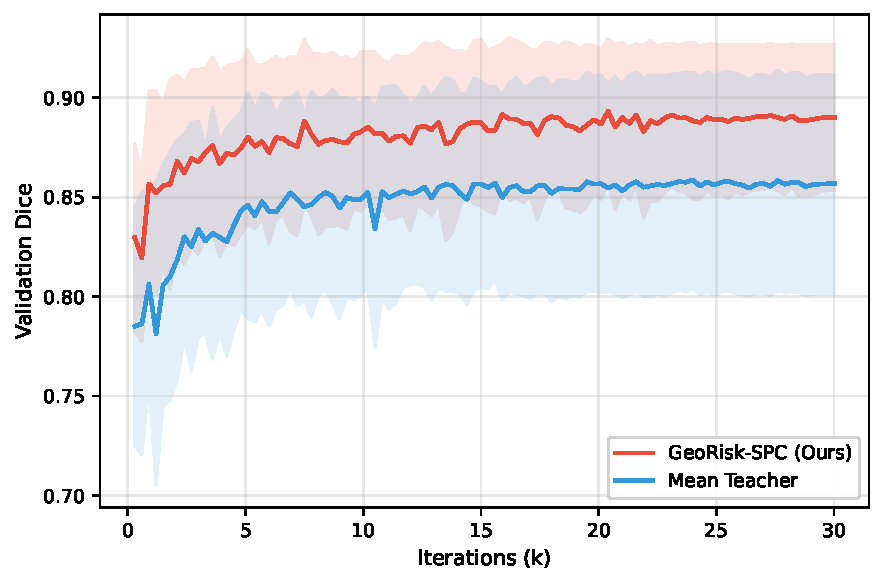
\includegraphics[width=\columnwidth]{figures/convergence.pdf}
\caption{Training curves of GeoRisk-SPC and Mean Teacher on EndoVis 2017 (40\% labeled data, 4-fold average). GeoRisk-SPC converges faster and achieves higher final Dice score. Shaded regions indicate standard deviation across folds.}
\label{fig:convergence}
\end{figure}

\begin{figure}[t]
\centering
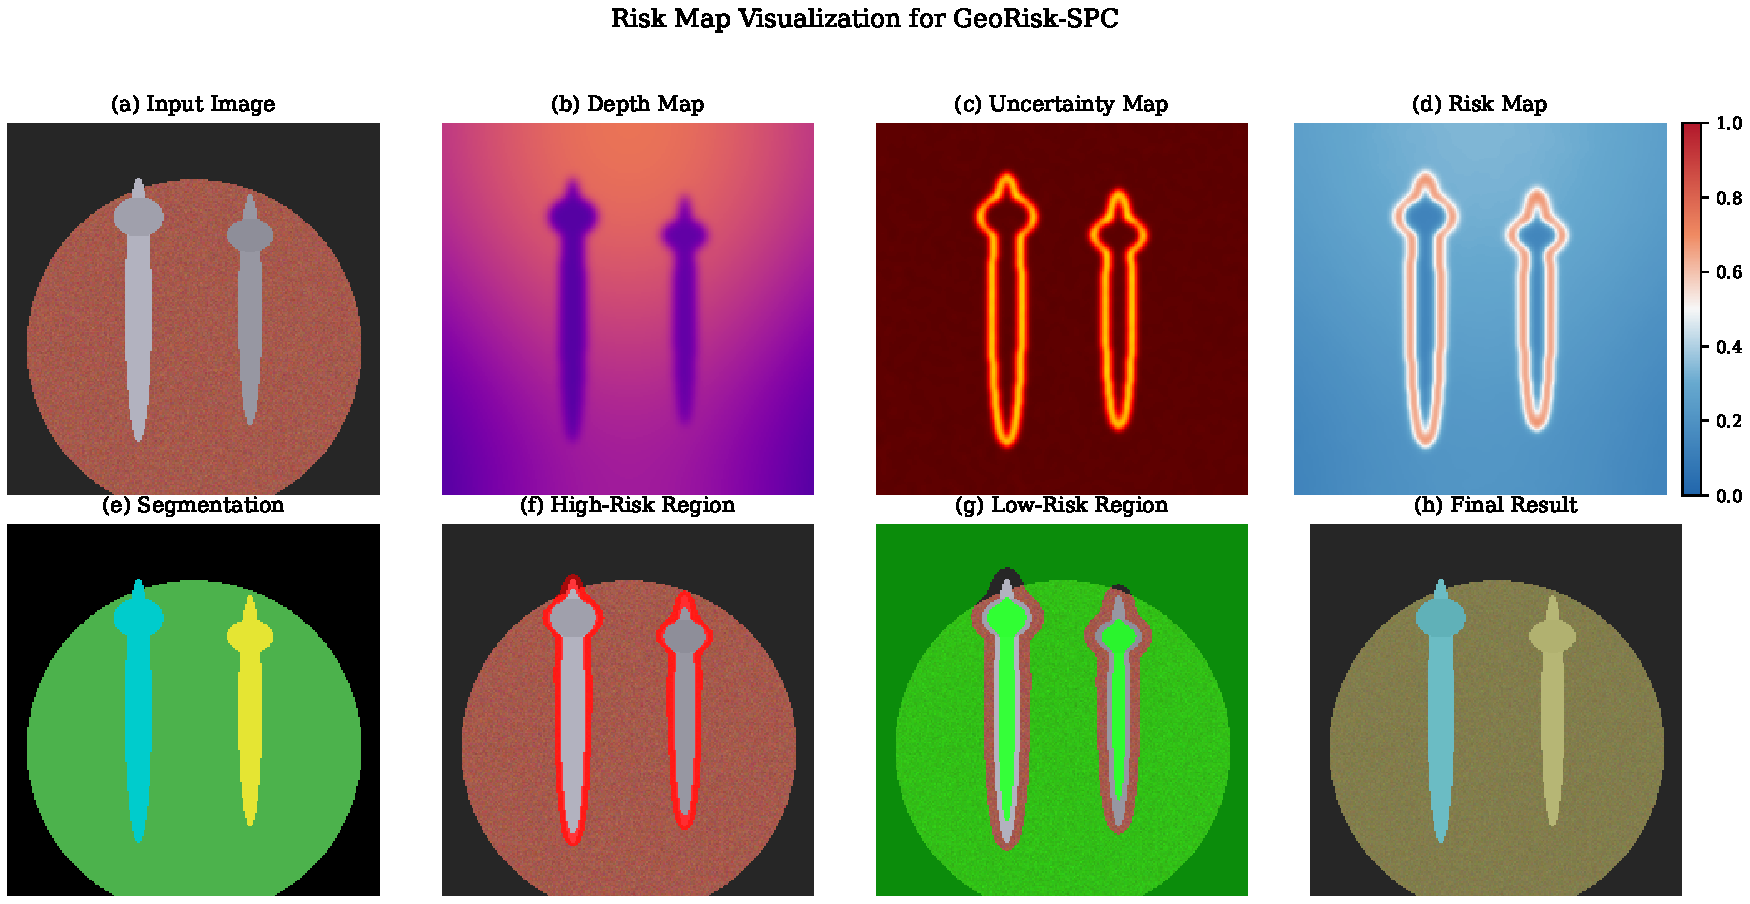
\includegraphics[width=\columnwidth]{figures/risk_map.pdf}
\caption{Visualization of risk maps. From left to right: input image, depth map, risk map, and segmentation result. High-risk regions (red) correspond to instrument boundaries and ambiguous areas.}
\label{fig:risk_map}
\end{figure}

\subsubsection{Selective Depth Feature Usage}
Figure~\ref{fig:depth_usage} visualizes the depth feature activations at each encoder level of the DepthGuiderV4 module across three test samples. Each row corresponds to a different input case, showing the depth encoder output (\textit{depth\_feat}) and geometry encoder output (\textit{geom\_feat}) at layers L0--L4.

A striking pattern emerges: depth features are actively utilized at shallow layers (L0--L2) but suppressed to near-zero at deep layers (L3--L4). At L0 (16 channels, $224\times224$), depth features exhibit strong spatial activations with values up to 2.88, indicating rich geometric information is being extracted. L1 and L2 maintain meaningful activations (max values 1.52 and 1.36 respectively). In contrast, L3 and L4 show near-zero activations (max $< 10^{-4}$), effectively learning to ignore depth input.

This selective usage pattern has a natural interpretation. Shallow layers are responsible for capturing fine-grained details such as edges, textures, and boundaries---precisely where geometric information from depth discontinuities is most valuable for distinguishing instrument edges from tissue boundaries. Deep layers encode high-level semantic features where the category information suffices and depth cues provide diminishing marginal returns. The model learns this ``use depth at shallow layers, ignore it at deep layers'' strategy autonomously, without explicit supervision to do so.

This finding also validates the design of our risk localization module, which computes depth discontinuity at the input resolution---where the raw geometric signal is strongest---rather than at deep feature levels. The DepthGuiderV4 module further enhances this by fusing depth features at each encoder level, allowing the network to selectively attend to geometric cues where they are most informative.

\begin{figure}[t]
\centering
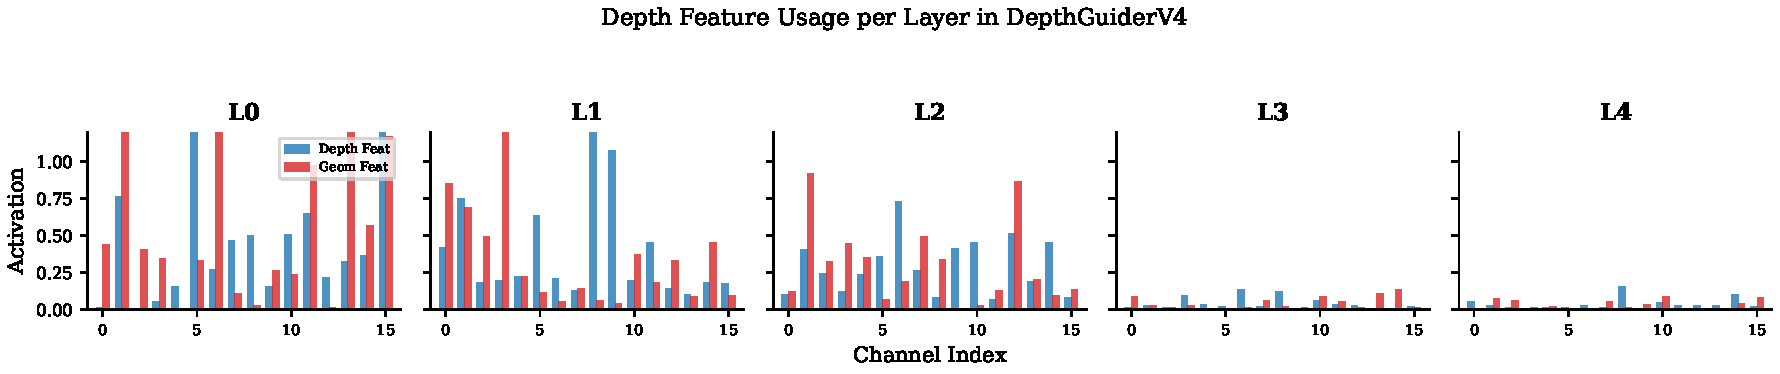
\includegraphics[width=\columnwidth]{figures/depth_usage_per_layer.pdf}
\caption{Depth feature activations per encoder layer in DepthGuiderV4. Each row shows a test sample with the input image overlaid with depth (column 1) and depth encoder outputs at layers L0--L4 (columns 2--6). Shallow layers (L0--L2) show active depth feature extraction, while deep layers (L3--L4) learn to suppress depth contributions (gray regions marked ``OFF''). This selective usage pattern indicates that geometric cues are most beneficial for capturing fine-grained boundary details rather than high-level semantics.}
\label{fig:depth_usage}
\end{figure}

\section{Discussion}

\subsection{Why Geometry-conditioned Risk Supervision Works}
The effectiveness of our approach stems from two complementary insights. First, pseudo-label reliability is spatially heterogeneous in surgical scenes: instrument boundaries exhibit complex 3D geometry, motion blur, tissue deformation, and specular reflections that make pseudo-labels unreliable. Second, this heterogeneity correlates with geometric structure—depth discontinuities from monocular depth estimation coincide with instrument boundaries, providing an external structural cue for identifying unreliable regions.

Once risk is localized, differentiated supervision becomes possible: hard pseudo-labels in reliable regions provide strong learning signals, while soft structural consistency in high-risk regions prevents error propagation. This is more effective than either uniformly trusting all pseudo-labels (which propagates errors) or uniformly downweighting them (which wastes reliable signals).

\subsection{Computational Overhead}
GeoRisk-SPC introduces minimal computational overhead. The risk localization module adds approximately 5\% to the training time compared to standard Mean Teacher. The dual-decoder architecture increases memory usage by about 30\%, but this is offset by the improved convergence speed (fewer iterations needed to reach optimal performance).

\subsection{Limitations}
Our method has several limitations:
\begin{itemize}
\item \textbf{Depth quality dependency}: The effectiveness of risk localization depends on the quality of pre-computed depth maps. Poor depth estimation may lead to inaccurate risk maps. Future work could explore using multiple depth estimators or uncertainty-aware depth fusion.
\item \textbf{Threshold sensitivity}: The performance is sensitive to the risk threshold $\tau_r$ and confidence threshold $\tau_c$. We provide ablation studies on threshold sensitivity (Table~\ref{tab:ablation}), but adaptive thresholding strategies could further improve robustness.
\item \textbf{Dataset scope}: We evaluated on EndoVis 2017 (binary segmentation). Validation on multi-class surgical datasets and other surgical scenarios is needed to confirm generalizability.
\item \textbf{Computational overhead}: The dual-decoder architecture increases memory usage by approximately 30\% compared to standard Mean Teacher, though this is offset by improved convergence speed.
\end{itemize}

\section{Conclusion}
We proposed GeoRisk-SPC, a geometry-conditioned pseudo-label risk supervision framework for semi-supervised surgical instrument segmentation. Our key insight is that pseudo-label reliability is spatially heterogeneous and correlates with geometric structure: depth discontinuities from monocular depth estimation reveal where pseudo-labels are unreliable. Based on this insight, we design a risk localization mechanism that partitions unlabeled pixels into low-risk and high-risk regions, applying hard pseudo-labels to reliable regions and soft structural consistency to ambiguous regions.

The full model GeoRisk-SPC-DG incorporates a depth-guided encoder with cross-attention fusion for enhanced geometric feature extraction. Experiments on EndoVis 2017 demonstrate that GeoRisk-SPC-DG achieves 89.78\% Dice at 40\% labels, 88.09\% at 10\% labels, and 86.89\% at 5\% labels, outperforming strong baselines UniMatch and SegMatch across all settings. Notably, GeoRisk-SPC-DG with 10\% labels surpasses SegMatch with 40\% labels, demonstrating that geometry-aware risk supervision enables superior label efficiency.

Future work includes extending our method to 3D surgical scene segmentation, exploring adaptive thresholding strategies for risk map generation, and validating on additional surgical datasets to confirm generalizability.

\section*{Acknowledgment}
This work was supported by ...

\bibliographystyle{IEEEtran}
\bibliography{references}

\end{document}
